\documentclass[journal,12pt,onecolumn]{IEEEtran}
\usepackage{cite}
 \usepackage{caption}
\usepackage{graphicx}
\usepackage{amsmath,amssymb,amsfonts,amsthm}
\usepackage{algorithmic}
\usepackage{graphicx}
\usepackage{textcomp}
\usepackage{xcolor}
\usepackage{txfonts}
\usepackage{listings}
\usepackage{enumitem}
\usepackage{mathtools}
\usepackage{gensymb}
\usepackage{comment}
\usepackage[breaklinks=true]{hyperref}
\usepackage{tkz-euclide} 
\usepackage{listings}
\usepackage{gvv}
%\def\inputGnumericTable{}                                 
\usepackage[latin1]{inputenc} 
\usetikzlibrary{arrows.meta, positioning}
\usepackage{xparse}
\usepackage{color}                                            
\usepackage{array}                                            
\usepackage{longtable}                                       
\usepackage{calc}                                             
\usepackage{multirow}
\usepackage{multicol}
\usepackage{hhline}                                           
\usepackage{ifthen}                                           
\usepackage{lscape}
\usepackage{tabularx}
\usepackage{array}
\usepackage{float}

\usepackage{float}
%\newcommand{\define}{\stackrel{\triangle}{=}}
\theoremstyle{remark}
\usepackage{circuitikz}
\captionsetup{justification=centering}
\usepackage{tikz}

\title{Matrices in Geometry 10.7.84}
\author{EE25BTECH11035 - Kushal B N}
\begin{document}
\vspace{3cm}
\maketitle
{\let\newpage\relax\maketitle}
\textbf{Question: }
Let $2x^2 + y^2 - 3xy = 0$ be the equation of pair of tangents drawn from the origin $\vec{O}$ to a circle of radius 3 with the centre in the first quadrant. If $\vec{A}$ is one of the points of contact, find the length of \textit{OA}.
\hfill (JEE 2001)

\textbf{Given: }\\
The equation of pair of tangents
\begin{equation}
    y^2 - 3xy + 2x^2 = 0
\end{equation}
Radius $r = 3$
\textbf{Solution: }\\
Factorising the given equation of pair of tangents
\begin{equation}
    (y-x)(y-2x) = 0
\end{equation}

The direction vectors of the two tangent lines from the origin 
\begin{equation}
    \vec{m}_1 = \myvec{1\\1}
\end{equation}
\begin{equation}
    \vec{m}_2 = \myvec{1\\2}
\end{equation}

Now, let $2\phi$ be the angle between the two tangent lines.
\begin{equation}
    \vec{m}_1^{\top}\vec{m}_2 = \myvec{1&1}\myvec{1\\2} = 3
\end{equation}

\begin{equation}
    \norm{\vec{m}_1} = \sqrt{\vec{m}_1^{\top}\vec{m}_1} = \sqrt{2}
\end{equation}

\begin{equation}
    \norm{\vec{m}_2} = \sqrt{\vec{m}_2^{\top}\vec{m}_2} = \sqrt{5}
\end{equation}

\begin{equation}
    \cos{2\phi} = \frac{\vec{m}_1^{\top}\vec{m}_2}{\norm{\vec{m}_1}\norm{\vec{m}_2}} = \frac{3}{\sqrt{2}\sqrt{5}} = \frac{3}{\sqrt{10}}
\end{equation}

\begin{equation}
    \implies \tan{2\phi} = \frac{\sqrt{1 - \cos^2{2\phi}}}{\cos{2\phi}} = \frac{1/\sqrt{10}}{3\sqrt{10}} = \frac{1}{3}
\end{equation}

Let the centre of the circle be $\vec{C}$, so that in the right-angled triangle $\Delta OAC$, we have (as $AC = r = 3$)
\begin{equation}
    \tan{\phi} = \frac{AC}{OA} = \frac{3}{OA}
\end{equation}

\begin{equation}
    \tan{2\phi} = \frac{2\tan{\phi}}{1 - \tan^2{\phi}}
\end{equation}
Let $t = \tan{\phi}$

\begin{equation}
    \frac{1}{3} = \frac{2t}{1 - t^2}
\end{equation}

\begin{equation}
    \implies t^2 + 6t -1 = 0
\end{equation}

Solving the above quadratic equation using the quadractic formula, we get

\begin{equation}
    t = -3 \pm \sqrt{10}
\end{equation}
Now, the angle being acute implies that $\tan{\phi} > 0$, so
\begin{equation}
    \tan{\phi} = \sqrt{10} - 3
\end{equation}

\begin{equation}
    \implies OA = \frac{3}{\tan{\phi}} = \frac{3}{\sqrt{10} - 3}
\end{equation}

Rationalising the denominator, we get
\begin{equation}
    \fbox{$OA = 9 + 3\sqrt{10}$}
\end{equation}

\textbf{Final Answer: }\\
$\therefore$ The length of $OA$ is equal to $9 + 3\sqrt{10}$ units.
\begin{figure}[H]
    \centering
    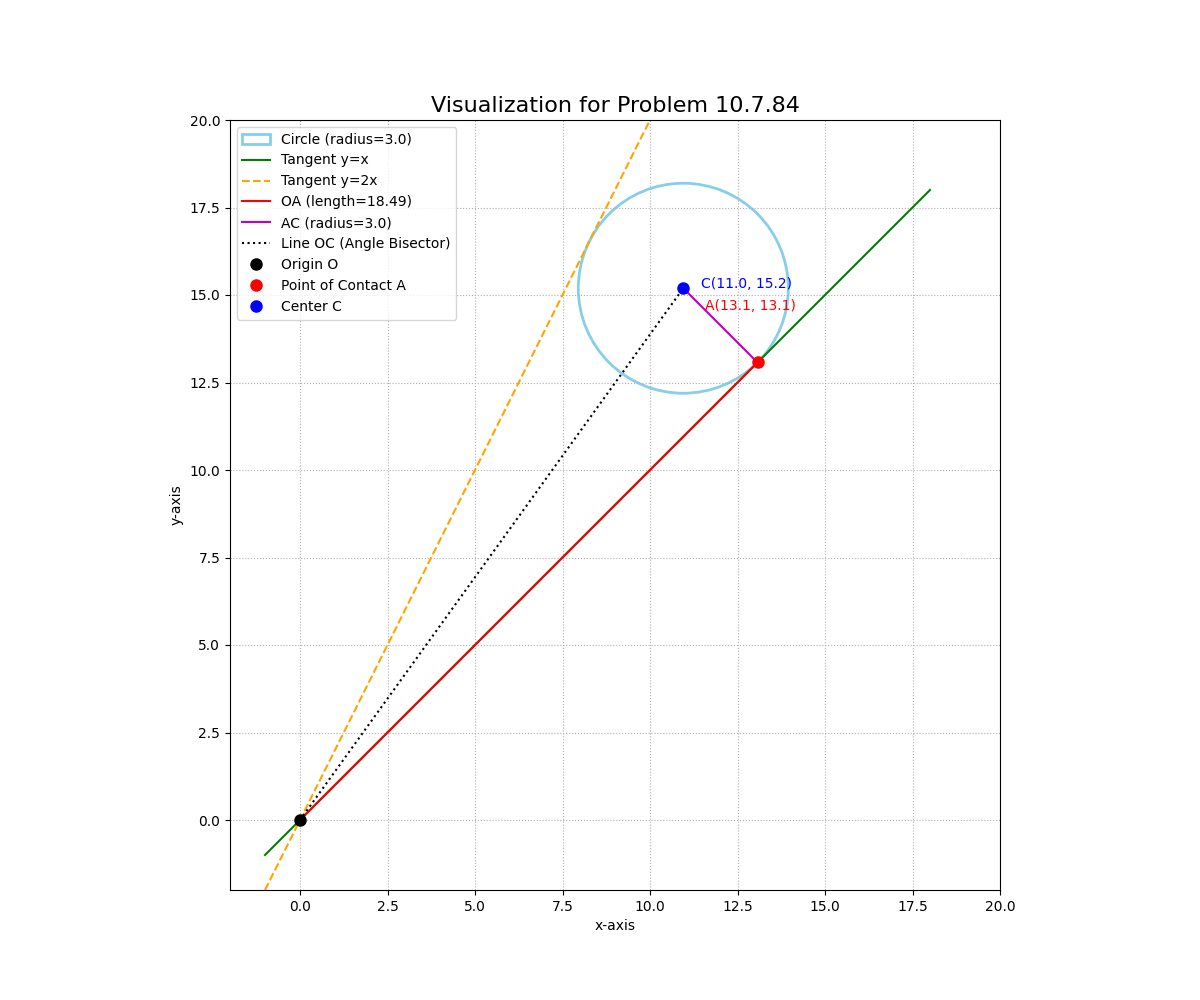
\includegraphics[width=0.60\columnwidth]{figs/2.png}
    \caption{Plot for 10.7.84}
\end{figure}
\end{document}
